\subsection{Artificial Neural Networks}
\textit{Artificial neural networks} (\textit{ANNs}), sometimes referred to as \textit{neural networks} (\textit{NNs}), are a category of bio-inspired algorithms that are structured like and can learn similarly to a brain. They are the foundation of many modern machine learning systems. Early concepts have been developed in 1943 \cite{first-neuron}, but were not widely applicable due to the lack of sufficient computational resources. However, today, even consumer-grade graphics cards intended for video games are powerful enough to run complex neural network models and are starting to be engineered specifically to accelerate machine learning applications \cite{tensor-cores}.

Commonly treated as a black box, artificial neural networks can be used as function approximators. Say, for example, we want to predict the output of a function $g$ without knowledge of its inner workings. Instead, we are only given several input-output samples produced by $g$. In this case, we may use a neural network, which, given a set of parameters $\theta$, also produces an input-output mapping $f_\theta$. This mapping, by default, is unlikely to accurately represent $g$. We now iteratively adjust $\theta$ using the input-output samples created by $g$ so that $f_\theta$ also produces a similar output for each given input. The network is then expected to behave much like $g$, even for previously unknown inputs.

The fundamental unit of a neural network is often the McCulloch-Pitts neuron \cite{first-neuron}. Inspired by biological neurons, McCulloch-Pitts mathematical neurons receive a vector of real-valued inputs $x = (x_1, ..., x_n)$, which are weighted with parameters $w = (w_1, ..., w_n)$ and then summed to produce a single, real-valued output. This output is then further transformed by an \textit{activation function} $h$, enabling the neuron to produce non-linear mappings. A \textit{threshold} term (or \textit{bias}) $b$ is usually introduced as well, forming the equation:
\begin{equation*}
    y = h\left(\sum_{i=1}^n w_i x_i + b \right)
\end{equation*}
Common activation functions include \textit{sigmoid}, \textit{tanh}, or \textit{ReLU}\footnote{Rectified Linear Unit}. The full neuron is visualized in Figure \ref{fig:neuron}.
\begin{figure}[ht]
    \centering
    \begin{subfigure}{0.49\textwidth}
        \raggedright
        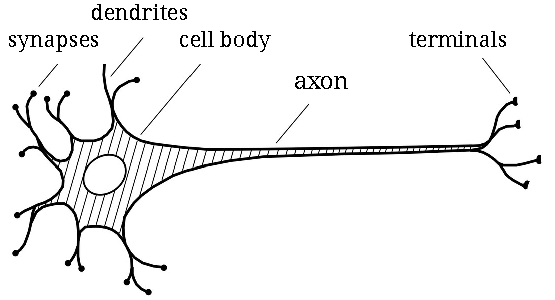
\includegraphics[width=\textwidth]{assets/bio_neuron.pdf}
    \end{subfigure}
    \begin{subfigure}{0.5\textwidth}
        \raggedleft
        \begin{tikzpicture}
            \node (x1) {$x_1$};
            \node [below = 0.25 of x1] (x2) {$x_2$};
            \node [below = 0.25 of x2] (x3) {$x_3$};
            \node [below = 0.15 of x3] (xdot) {\vdots};
            \node [below = 0.35 of xdot] (xn) {$x_n$};

            \node [right = of x3, draw, circle] (sum) {$\sum$};

            \node [above = of sum] (bias) {$b$};

            \node [right = 0.5 of sum, draw, rectangle] (activation) {$h$};
            \node [right = of activation] (y) {$y$};

            \draw [->] (x1) -- (sum);
            \draw [->] (x2) -- (sum);
            \draw [->] (x3) -- (sum);
            \draw [->] (xn) -- (sum);

            \draw [->] (bias) -- (sum);

            \draw [->] (sum) -- (activation);
            \draw [->] (activation) -- (y);
        \end{tikzpicture}
    \end{subfigure}
    \caption{Comparison of a biological neuron \cite{bio-neuron} (left) and a mathematical McCulloch-Pitts neuron (right).}
    \label{fig:neuron}
\end{figure}
Individual neuron units were later put together to form the \textit{perceptron} \cite{first-perceptron}. Multiple layers of neurons are called a \textit{multi-layer perceptron}. Having many of such layers popularized the terms \textit{deep neural network} and \textit{deep learning}. These types of perceptrons can be expressed using a series of matrix and vector multiplications and additions
\begin{equation*}
    f(x) = h_n \left(W_n \dots h_2\left( W_2 h_1(W_1x + b_1) + b_2 \right) \dots + b_n\right),
\end{equation*}
where $W_1, \dots, W_n$ are weight matrices, $b_1, \dots, b_n$ are bias vectors and $h_1, \dots, h_n$ are activation functions for each layer. Note that the input vector $x$ is mapped to another vector $f(x)$, which may have a different number of dimensions.

Perceptrons can be trained using gradient descent of an \textit{error} (or \textit{loss}) term with respect to its parameters $\theta$, which is referred to as \textit{back-propagation} \cite{back-propagation}. Calculating gradients for each neuron in a complex model is difficult and must be highly optimized. Programming libraries such as \mbox{\textit{TensorFlow}} \cite{tensorflow} or \textit{PyTorch} \cite{pytorch} solve this issue by performing automatic differentiation and parallelizing mathematical operations on the GPU.
